% Left graph of Figure 2 in Kilbertus et al. (2017), from Hardt et al. (2016): A reaches the
% prediction only through the resolving variable X_1, so there is no unresolved discrimination.
% Compile on its own (pdflatex same-distribution-graph-a.tex); the thesis includes the PDF.
% Same styles as scm-running-example.tex; graphs (a) and (b) share their node positions, so both
% PDFs have the same size.
\documentclass[12pt,border=2pt]{standalone}
\usepackage[T1]{fontenc}
\usepackage{mathpazo}
\usepackage{tikz}
\usetikzlibrary{arrows.meta}
\begin{document}
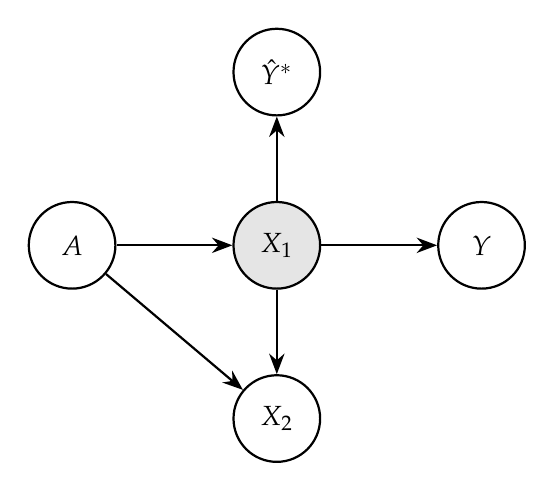
\begin{tikzpicture}[
    var/.style        = {circle, draw, thick, minimum size=11mm, inner sep=0pt},
    resolving/.style  = {var, fill=gray!20},
    arr/.style        = {-{Stealth[length=2.6mm]}, thick},
    unresolved/.style = {arr, red!70!black}
  ]
  \node[var]       (A)  at (0, 0)    {$A$};
  \node[resolving] (X1) at (2.6, 0)  {$X_1$};
  \node[var]       (Y)  at (5.2, 0)  {$Y$};
  \node[var]       (R)  at (2.6, 2.2)  {$\hat{Y}^{*}$};
  \node[var]       (X2) at (2.6, -2.2) {$X_2$};

  \draw[arr] (A) -- (X1);
  \draw[arr] (X1) -- (R);
  \draw[arr] (X1) -- (Y);
  \draw[arr] (X1) -- (X2);
  \draw[arr] (A) -- (X2);
\end{tikzpicture}
\end{document}
